% !TeX root = ../main.tex
% Add the above to each chapter to make compiling the PDF easier in some editors.

\chapter{Implementation of the model}\label{chapter:implementation_of_the_model}

\section{Data Loader}

Now that we have a better understanding of how Gen6D operates, we're interested in testing it with the synthetic images from the \textsc{SpaceCraft} dataset. To accomplish this, we need to redefine the Data Loader to supply the model with the necessary data in the required format. In the file \texttt{database.py}, located in the \texttt{Gen6D/dataset} directory, there is an \ac{ABC} named \texttt{BaseDatabase()} containing all the essential methods, as shown in the code below:

\bigbreak

\begin{lstlisting}[style=pythonstyle, label=lst:0, caption={Python code of \ac{ABC} \texttt{BaseDatabase()}, from file \texttt{database.py}.}]
	class BaseDatabase(abc.ABC):
    def __init__(self, database_name):
        self.database_name = database_name

    @abc.abstractmethod
    def get_image(self, img_id):
        pass

    @abc.abstractmethod
    def get_K(self, img_id):
        pass

    @abc.abstractmethod
    def get_pose(self, img_id):
        pass

    @abc.abstractmethod
    def get_img_ids(self):
        pass

    def get_mask(self,img_id):
        # dummy mask
        img = self.get_image(img_id)
        h, w = img.shape[:2]
        return np.ones([h,w],np.bool_)
\end{lstlisting}

\bigbreak

Our goal, therefore, is to write a new class that inherits from the \ac{ABC} \\\texttt{BaseDatabase()}, and implement each abstract method in the same manner as it was done for the \textsc{Linemod} and \textsc{GenMOP} datasets, for example. We will also adapt the code in various places, especially in the \texttt{eval.py} file, to ensure compatibility with the \textsc{SpaceCraft} dataset. The Python code for the new data loading class \texttt{SpaceCraftCVLabDatabase()} can be found in Listing~\ref{lst:1}.

\section{From Quaternions to Rotation Matrices}
\fancyhead[C]{\small\textsc{3.2. From Quaternions to Rotation Matrices}}

In Gen6D, the model represents the ground truth and estimated poses using the format ${\bm{\mathrm{P}}}=(\bm{\mathrm{R}},\,\bm{\mathrm{t}})$. Here, $\bm{\mathrm{R}}$ denotes the rotation matrix and $\bm{\mathrm{t}}$ is the translation vector.
The thing is, in the \textsc{SpaceCraft} dataset, the poses have the format ${\bm{\mathrm{P}}}=(\underline{\bm{\mathrm{q}}},\,\bm{\mathrm{t}})$, where $\underline{\bm{\mathrm{q}}}$ is a \textit{quaternion}. We use quaternions for three-dimensional rotation calculations because they offer several benefits over rotation matrices. Notably, quaternions are more compact, requiring only four elements to be stored compared to nine for a matrix. Additionally, they are more efficient when composing rotations thanks to their algebraic properties.

Despite the benefits of quaternions mentioned earlier, other datasets frequently represent poses using a combination of rotation matrices and translation vectors. Therefore, to align with Gen6D's pose format, this section will focus on converting quaternions into rotation matrices \cite{jia2022quaternions}.

\bigbreak 

Quaternions were first introduced by the Irish mathematician W. R. Hamilton in 1843 as an extension of the complex numbers \cite{Hamilton1866}. In the first place, we provide the definition of a \textit{quaternion} $\underline{\bm{\mathrm{q}}}$: it is the sum of a scalar $\mathrm{q}_0$ and a vector $\bm{\mathrm{q}}=(\mathrm{q}_1, \mathrm{q}_2, \mathrm{q}_3)$, that is,
\begin{center}
	$\underline{\bm{\mathrm{q}}} \stackrel{\text{def.}}{=} \mathrm{q}_0 + \bm{\mathrm{q}} = \mathrm{q}_0 + \mathrm{q}_1\bm{i} + \mathrm{q}_2\bm{j} + \mathrm{q}_3\bm{k}$.
\end{center}

\noindent In the above, $\bm{i}$, $\bm{j}$ and $\bm{k}$ denote the three unit vectors of the canonical basis for 
the set of all ordered triples of real numbers $\mathbb{R}^3$. The set of quaternions is denoted by the 4-space $\mathbb{H}$.

\bigbreak 
The quaternion addition is component-wise. Regarding the product of two quaternions, it is essential to first outline the foundational rule established by \mbox{Hamilton}:
\begin{align*}
	\bm{i}^2 &= \bm{j}^2 = \bm{k}^2 = \bm{ijk}= -1.
\end{align*}

\noindent We derive the following multiplication table:

\begin{center}
\setlength{\arrayrulewidth}{1pt}
\renewcommand{\arraystretch}{1.2}
\begin{tabular}{|m{1.5em}||m{1.5em}|m{1.5em}|m{1.5em}|m{1.5em}|}
    \hline
    \rowcolor{gray!25}
    \cellcolor{gray!60}$\times$ & \centering $1$ & \centering $\bm{i}$ & \centering $\bm{j}$ & \centering $\bm{k}$ \tabularnewline
    \hline\hline
    \cellcolor{gray!25}$1$ & \centering $1$ & \centering $\bm{i}$ & \centering $\bm{j}$ & \centering $\bm{k}$ \tabularnewline
    \hline
    \cellcolor{gray!25}$\bm{i}$ & \centering $\bm{i}$ & \centering $-1$ & \centering $\bm{k}$ & \centering $-\bm{j}$ \tabularnewline
    \hline
    \cellcolor{gray!25}$\bm{j}$ & \centering $\bm{j}$ & \centering $-\bm{k}$ & \centering $-1$ & \centering $\bm{i}$ \tabularnewline
    \hline
    \cellcolor{gray!25}$\bm{k}$ & \centering $\bm{k}$ & \centering $\bm{j}$ & \centering $-\bm{i}$ & \centering $-1$ \tabularnewline
    \hline
\end{tabular}
\end{center}

\bigbreak 

\noindent Let $(\underline{\bm{\mathrm{p}}}, \underline{\bm{\mathrm{q}}})\in\mathbb{H}^2$, we are now able to present the multiplication of $\underline{\bm{\mathrm{p}}}$ and $\underline{\bm{\mathrm{q}}}$:
\begin{align*}
    \underline{\bm{\mathrm{p}}}\underline{\bm{\mathrm{q}}} &= \underbrace{\mathrm{p}_0\mathrm{q}_0 - \bm{\mathrm{p}} \cdot \bm{\mathrm{q}}}_{\text{scalar part}} + \underbrace{\mathrm{p}_0\bm{\mathrm{q}} + \mathrm{q}_0\bm{\mathrm{p}} + \bm{\mathrm{p}} \times \bm{\mathrm{q}}}_{\text{vector part}}.
\end{align*}

\noindent In the preceding, we recall that the binary operation $\mathbb{R}^3\times\mathbb{R}^3\rightarrow\mathbb{R}$ : $(\bm{\mathrm{p}},\bm{\mathrm{q}})\mapsto\bm{\mathrm{p}}\cdot\bm{\mathrm{q}}\stackrel{\text{def.}}{=}\bm{\mathrm{p}}^\intercal\bm{\mathrm{q}}$ is the \textit{dot product}, and the other
\begin{align*}
	\mathbb{R}^3\times\mathbb{R}^3\rightarrow\mathbb{R}^3 : (\bm{\mathrm{p}},\bm{\mathrm{q}})\mapsto\bm{\mathrm{p}}\times\bm{\mathrm{q}}\stackrel{\text{def.}}{=}\begin{vmatrix} \bm{i} & \bm{j} & \bm{k} \\ \mathrm{p}_1 & \mathrm{p}_2 & \mathrm{p}_3 \\
		\mathrm{q}_1 & \mathrm{q}_2 & \mathrm{q}_3 \end{vmatrix}
		=[\bm{\mathrm{p}}]_{_{_\times}}\bm{\mathrm{q}}
\end{align*}

\noindent is the \textit{cross product}, and the operator $[\bm{\mathrm{p}}]_{_{_\times}}$yields the transformation matrix that when multiplied from the right with a vector $\bm{\mathrm{q}}$ gives $\bm{\mathrm{p}}\times\bm{\mathrm{q}}$.
\bigbreak 
Several additional definitions are essential before we can begin the conversion of quaternions to rotation matrices. 


\noindent Let $\underline{\bm{\mathrm{q}}}=\mathrm{q}_0 + \bm{\mathrm{q}}$ be a quaternion. The \textit{complex conjugate} of $\underline{\bm{\mathrm{q}}}$, denoted by $\underline{\bm{\mathrm{q}}}^\star$, is given by the map
\begin{align*}
	\mathbb{H}\rightarrow\mathbb{H}:\underline{\bm{\mathrm{q}}}\mapsto\underline{\bm{\mathrm{q}}}^\star\stackrel{\text{def.}}{=}\mathrm{q}_0 - \bm{\mathrm{q}}.
\end{align*} 

\noindent The \textit{norm} of a quaternion $\underline{\bm{\mathrm{q}}}$, denoted $|\underline{\bm{\mathrm{q}}}|$, is the distance obtained from the map 
\begin{align*}
	\mathbb{H}\rightarrow\mathbb{R}^+:\underline{\bm{\mathrm{q}}}\mapsto|\underline{\bm{\mathrm{q}}}|\stackrel{\text{def.}}{=}\sqrt{\underline{\bm{\mathrm{q}}}^\star\underline{\bm{\mathrm{q}}}}.
\end{align*} 
Note that a quaternion whose norm is 1 is referred to as a \textit{unit quaternion}. The \textit{reciprocal} of a quaternion is defined as the map
\begin{align*}
	\mathbb{H}^*\rightarrow\mathbb{H}^*:\underline{\bm{\mathrm{q}}}\mapsto\underline{\bm{\mathrm{q}}}^{-1}\stackrel{\text{def.}}{=}\frac{\underline{\bm{\mathrm{q}}}^\star}{|\underline{\bm{\mathrm{q}}}|^2}.
\end{align*} 
We observe that if $\underline{\bm{\mathrm{q}}}$ is a unit quaternion, we simply have $\underline{\bm{\mathrm{q}}}^{-1}=\underline{\bm{\mathrm{q}}}^\star$. Furthermore, the subsequent proposition is accepted: if $\underline{\bm{\mathrm{q}}}$ is a unit quaternion, there exists a unique $\theta\in[0,2\pi]$ such that
\begin{align*}
	\underline{\bm{\mathrm{q}}} = \mathrm{q}_0 + \bm{\mathrm{q}}=\cos\frac{\theta}{2}+\bm{\mathrm{u}}\,\sin\frac{\theta}{2}\,,
\end{align*}
where the unit vector $\bm{\mathrm{u}}$ is defined as $\bm{\mathrm{u}}\stackrel{\text{def.}}{=}\frac{\bm{\mathrm{q}}}{|\bm{\mathrm{q}}|}$.

\setlength{\belowdisplayskip}{0.15cm}

\paragraph{Quaternion Rotation Operator} Let $\underline{\bm{\mathrm{q}}}\in\mathbb{H}$ be a unit quaternion, and let $\bm{\mathrm{v}}\in\mathbb{R}^3$ be a vector. The action of the $L_{\underline{\bm{\mathrm{q}}}}$ function 
\begin{align*}
	\mathbb{R}^3\rightarrow\mathbb{R}^3:\bm{\mathrm{v}}\mapsto L_{\underline{\bm{\mathrm{q}}}}(\bm{\mathrm{v}}) \stackrel{\text{def.}}{=} \underline{\bm{\mathrm{q}}}\bm{\mathrm{v}}\underline{\bm{\mathrm{q}}}^\star
\end{align*}
on $\bm{\mathrm{v}}$ is equivalent to a rotation of the vector through an angle $\theta$ about the axis of rotation $\bm{\mathrm{u}}$.

\setlength{\belowdisplayskip}{0.3cm}

\bigskip At last, we can proceed with our conversion task: our aim is to find a $3\times3$ rotation matrix $\bm{\mathrm{R}}$, such that
\begin{align*}
\left\{
    \begin{aligned}
    	L_{\bm{\mathrm{R}}}(\bm{\mathrm{v}}) &\stackrel{\text{def.}}{=} \bm{\mathrm{R}}\bm{\mathrm{v}} \\
        L_{\bm{\mathrm{R}}}(\bm{\mathrm{v}}) &= L_{\underline{\bm{\mathrm{q}}}}(\bm{\mathrm{v}}),
    \end{aligned}
\right.
\end{align*}

\noindent which means we wish to obtain an expression for $\bm{\mathrm{R}}$ by manipulating $L_{\underline{\bm{\mathrm{q}}}}\,$, utilizing principles of linear algebra and vector calculus. We consider the vector $\bm{\mathrm{v}}$ as a quaternion with a zero scalar component:


\begin{align*}
    L_{\underline{\bm{\mathrm{q}}}}(\bm{\mathrm{v}}) &= \underline{\bm{\mathrm{q}}}\bm{\mathrm{v}}\underline{\bm{\mathrm{q}}}^\star \\
    &= (\mathrm{q}_0+\bm{\mathrm{q}})(0+\bm{\mathrm{v}})(\mathrm{q}_0-\bm{\mathrm{q}}) \\
    &= (\underbrace{-\bm{\mathrm{q}}\cdot\bm{\mathrm{v}}}_{\text{scalar part}} + \underbrace{\mathrm{q}_0\bm{\mathrm{v}}+\bm{\mathrm{q}}\times\bm{\mathrm{v}}}_{\text{vector part}})(\mathrm{q}_0-\bm{\mathrm{q}}) \\
    &= \mathrm{q}_0(-\bm{\mathrm{q}}\cdot\bm{\mathrm{v}}) - (\mathrm{q}_0\bm{\mathrm{v}}+\bm{\mathrm{q}}\times\bm{\mathrm{v}})\cdot(-\bm{\mathrm{q}}) \\
    &\quad + (-\bm{\mathrm{q}}\cdot\bm{\mathrm{v}})(-\bm{\mathrm{q}}) + \mathrm{q}_0(\mathrm{q}_0\bm{\mathrm{v}}+\bm{\mathrm{q}}\times\bm{\mathrm{v}}) \\
    &\quad + (\mathrm{q}_0\bm{\mathrm{v}}+\bm{\mathrm{q}}\times\bm{\mathrm{v}})\times(-\bm{\mathrm{q}}) \\
    &= \underbrace{\cancel{-\mathrm{q}_0(\bm{\mathrm{q}}\cdot\bm{\mathrm{v}}) + \mathrm{q}_0(\bm{\mathrm{q}}\cdot\bm{\mathrm{v}})}}_{\text{scalar part}} \\
    &\quad + \underbrace{\bm{\mathrm{q}}\,(\bm{\mathrm{q}}\cdot\bm{\mathrm{v}}) + {\mathrm{q}_0}^2\,\bm{\mathrm{v}} + \mathrm{q}_0(\bm{\mathrm{q}}\times\bm{\mathrm{v}}) + \bm{\mathrm{q}}\times(\mathrm{q}_0\bm{\mathrm{v}}+\bm{\mathrm{q}}\times\bm{\mathrm{v}})}_{\text{vector part}} \\
    &= \bm{\mathrm{q}}\,(\bm{\mathrm{q}}^\intercal\bm{\mathrm{v}}) + {\mathrm{q}_0}^2\,\bm{\mathrm{v}} + \mathrm{q}_0(\bm{\mathrm{q}}\times\bm{\mathrm{v}}) + \bm{\mathrm{q}}\times(\mathrm{q}_0\bm{\mathrm{v}}+\bm{\mathrm{q}}\times\bm{\mathrm{v}}) \\
    &= (\bm{\mathrm{q}}\otimes\bm{\mathrm{q}} + {\mathrm{q}_0}^2\,\bm{\mathrm{I}}_{3\times3} + 2\,\mathrm{q}_0\,[\bm{\mathrm{q}}]_{_{_\times}}\!\! + [\bm{\mathrm{q}}]_{_{_\times}}^2)\,\,\bm{\mathrm{v}}
\end{align*}

\noindent In the above, $\otimes$ stands for the \textit{outer product} and $\bm{\mathrm{I}}_{3\times3}$ is the \textit{identity matrix}. 

\noindent Since $L_{\bm{\mathrm{R}}}(\bm{\mathrm{v}}) = L_{\underline{\bm{\mathrm{q}}}}(\bm{\mathrm{v}})$, we can identify $\bm{\mathrm{R}}$ as  $(\bm{\mathrm{q}}\otimes\bm{\mathrm{q}} + {\mathrm{q}_0}^2\,\bm{\mathrm{I}}_{3\times3} + 2\,\mathrm{q}_0\,[\bm{\mathrm{q}}]_{_{_\times}}\!\! + [\bm{\mathrm{q}}]_{_{_\times}}^2)$. We develop and simplify $\bm{\mathrm{R}}$ to find its final expression:

\begin{align*}
	\bm{\mathrm{R}} &= \bm{\mathrm{q}}\otimes\bm{\mathrm{q}} + {\mathrm{q}_0}^2\,\bm{\mathrm{I}}_{3\times3} + 2\,\mathrm{q}_0\,[\bm{\mathrm{q}}]_{_{_\times}}\!\! + [\bm{\mathrm{q}}]_{_{_\times}}^2 \\
	&= \begin{bmatrix}
    	{\mathrm{q}_1}^2 & \mathrm{q}_1\mathrm{q}_2 & \mathrm{q}_1\mathrm{q}_3 \\
    	\mathrm{q}_2\mathrm{q}_1 & {\mathrm{q}_2}^2 & \mathrm{q}_2\mathrm{q}_3 \\
    	\mathrm{q}_3\mathrm{q}_1 & \mathrm{q}_3\mathrm{q}_2 & {\mathrm{q}_3}^2
		\end{bmatrix} 
		+ {\mathrm{q}_0}^2
		\begin{bmatrix}
    	1 & 0 & 0 \\
    	0 & 1 & 0 \\
    	0 & 0 & 1
		\end{bmatrix}
		+
		2\,\mathrm{q}_0 \begin{bmatrix}
    	0 & -\mathrm{q}_3 & \mathrm{q}_2 \\
    	\mathrm{q}_3 & 0 & -\mathrm{q}_1 \\
    	-\mathrm{q}_2 & \mathrm{q}_1 & 0
		\end{bmatrix} \\
		&\quad+
		\begin{bmatrix}
    	0 & -\mathrm{q}_3 & \mathrm{q}_2 \\
    	\mathrm{q}_3 & 0 & -\mathrm{q}_1 \\
    	-\mathrm{q}_2 & \mathrm{q}_1 & 0
		\end{bmatrix}
		\begin{bmatrix}
    	0 & -\mathrm{q}_3 & \mathrm{q}_2 \\
    	\mathrm{q}_3 & 0 & -\mathrm{q}_1 \\
    	-\mathrm{q}_2 & \mathrm{q}_1 & 0
		\end{bmatrix} \\\\
		&=2
		\begin{bmatrix}
    	({\mathrm{q}_0}^2+{\mathrm{q}_1}^2)-\frac{1}{2} & \mathrm{q}_1\mathrm{q}_2-\mathrm{q}_0\mathrm{q}_3 & \mathrm{q}_1\mathrm{q}_3+\mathrm{q}_0\mathrm{q}_2 \\
    	\mathrm{q}_1\mathrm{q}_2+\mathrm{q}_0\mathrm{q}_3 & ({\mathrm{q}_0}^2+{\mathrm{q}_2}^2)-\frac{1}{2} & \mathrm{q}_2\mathrm{q}_3-\mathrm{q}_0\mathrm{q}_1 \\
    	\mathrm{q}_1\mathrm{q}_3-\mathrm{q}_0\mathrm{q}_2 & \mathrm{q}_2\mathrm{q}_3+\mathrm{q}_0\mathrm{q}_1 & ({\mathrm{q}_0}^2+{\mathrm{q}_3}^2)-\frac{1}{2}
		\end{bmatrix}
\end{align*} 

\bigskip

\noindent This completes our derivation of the rotation matrix $\bm{\mathrm{R}}$. The Python code can be found in Listing~\ref{lst:4}.

\section{Inverted Masks}

During the initial testing of Gen6D on the \textsc{SpaceCraft} dataset, we noticed that the estimated poses were particularly inaccurate. Upon investigation, we discovered that in the reference images folder, the masks were incorrectly inverted: typically, one expects a white object on a black background, but it was the opposite (see Figure~\ref{fig:mask1} below).

After discussing this, we realized that this was actually an error in the current version of the dataset. Therefore, we needed to correct the masks we were using through a Python script utilizing the OpenCV library. The Python script can be found in Listing~\ref{lst:5}.

\fancyhead[C]{\small\textsc{3.3. Inverted Masks}}

\bigskip

\begin{figure}[h]
    \centering
    \begin{minipage}{0.45\linewidth}
        \centering
        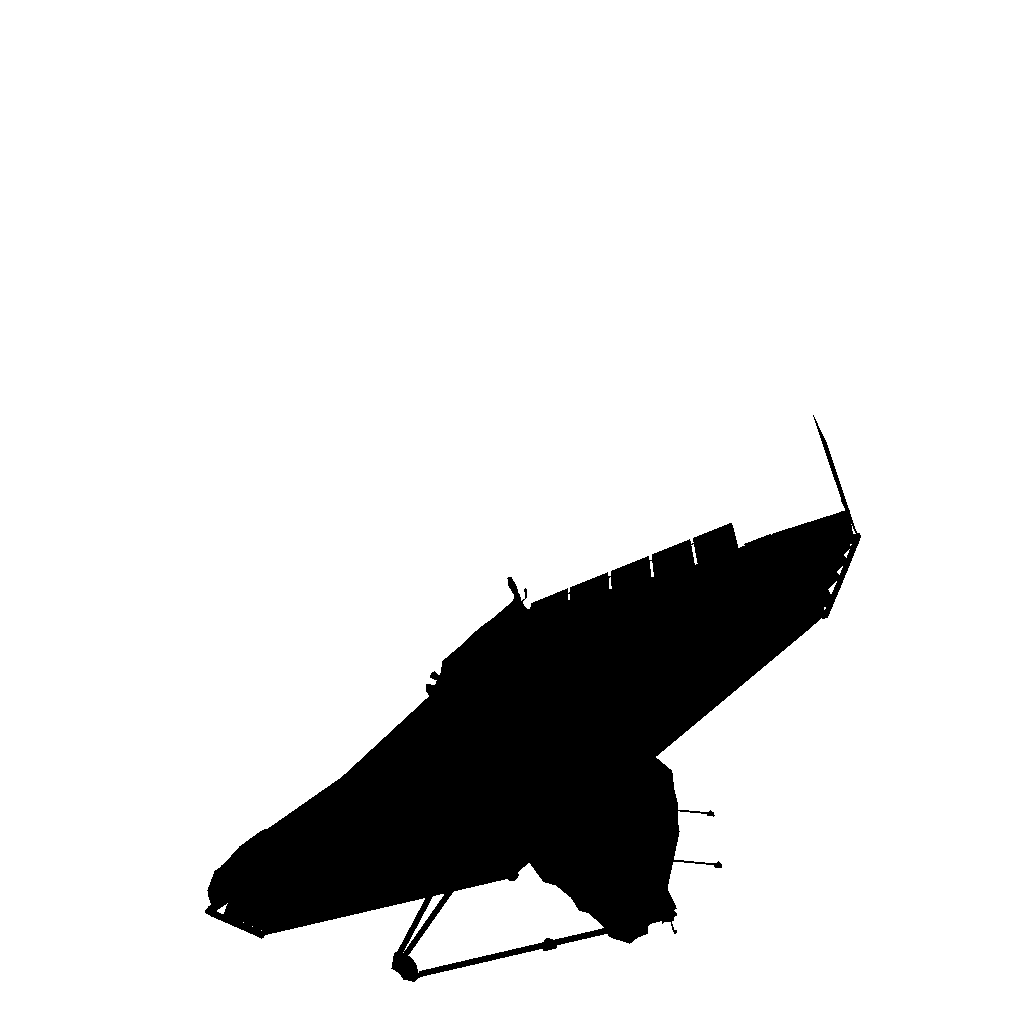
\includegraphics[width=\linewidth]{data/mask1.png} % First image
        \caption{James Webb Space Telescope, mask before the correction.}
        \label{fig:mask1}
    \end{minipage}\hfill
    \begin{minipage}{0.45\linewidth}
        \centering
        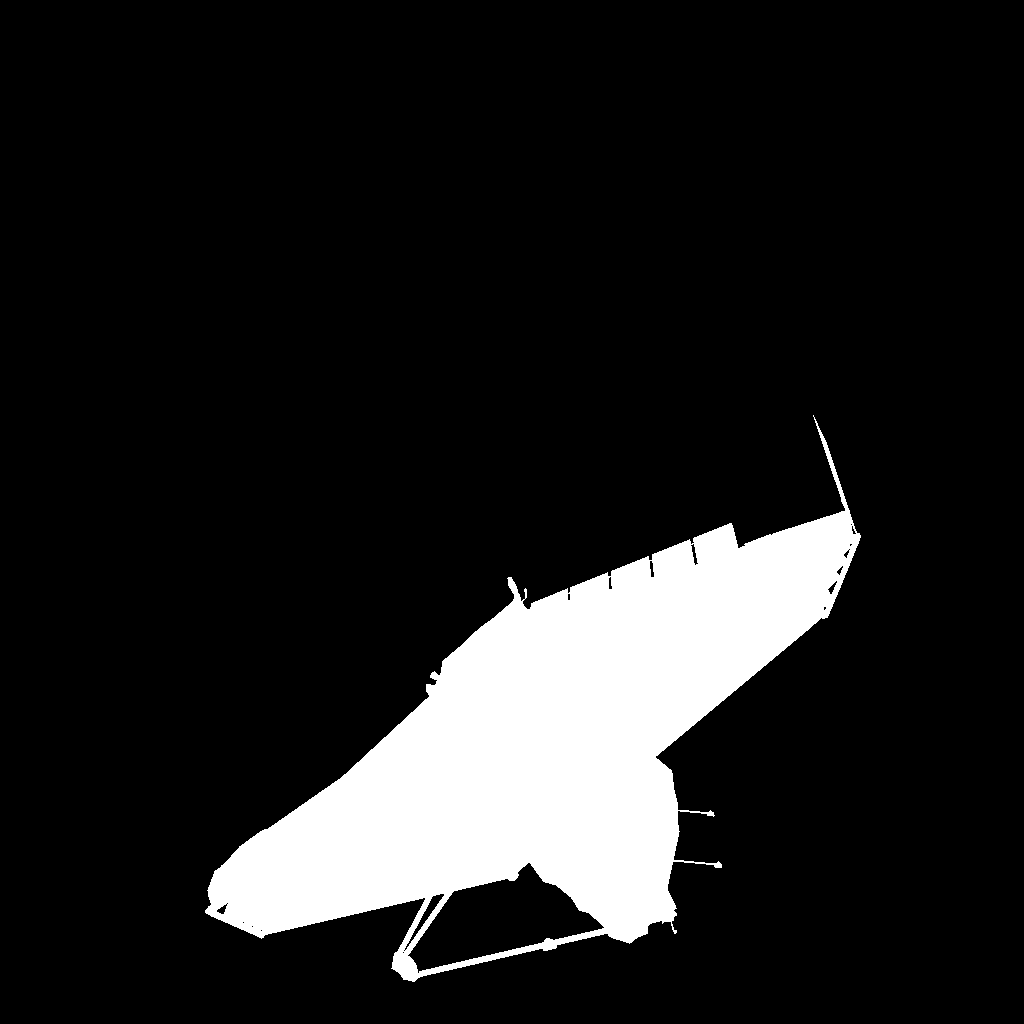
\includegraphics[width=\linewidth]{data/mask2.png} % Second image
        \caption{James Webb Space Telescope, mask after the correction using a script.}
        \label{fig:mask2}
    \end{minipage}
\end{figure}

\bigskip

\section{Resized Query Images}

During the initial testing of Gen6D, it became apparent that the deep learning model struggled when the object in the query image was either very large or very small (see Figure~\ref{fig:fig2} and Figure~\ref{fig:fig1} below). Consultation of the GitHub Issues section of the Gen6D repository revealed that this is a recurring problem: since the reference images are resized to $128\times 128$, the model's detector is trained to recognize an object in query images that ranges from half to double the size of the reference images, i.e., from $64\times 64$ to $256\times 256$.

\bigskip

Therefore, to improve the detector's results, resizing the query images is necessary. This is accomplished using a Python script that can be found in Listing~\ref{lst:6}. It's important to note that this adjustment also requires modifying the camera intrinsic matrix $\bm{\mathcal{K}}$ in the data loader, which converts points from the camera coordinate system to the pixel coordinate system.

\pagebreak

\fancyhead[C]{\small\textsc{3.4. Resized Query Images}}

\begin{figure}[H]
    \centering
    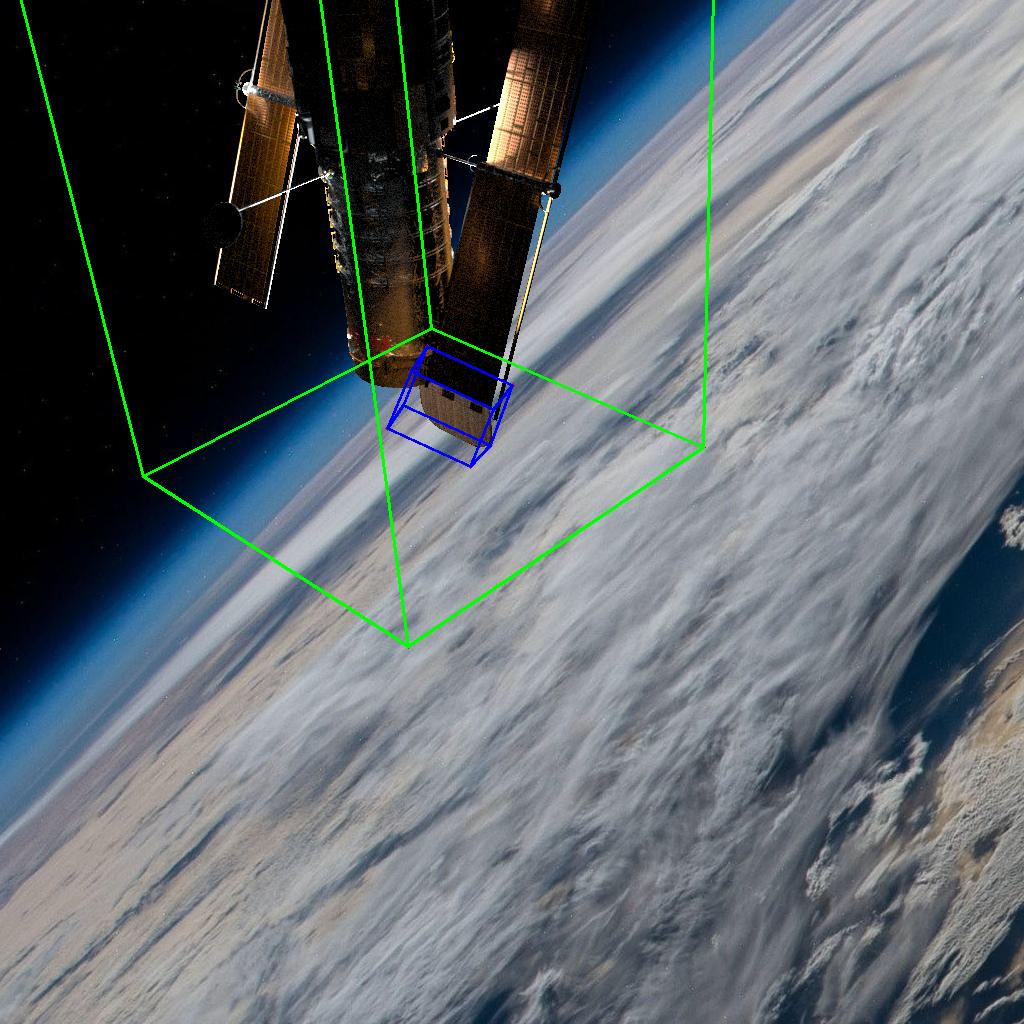
\includegraphics[width=0.70\linewidth]{data/fig2.jpg}
    \caption{Hubble Space Telescope with earth rendered background, 1024x1024 query image number 1, poor pose estimation (blue 3D bounding box) when the object inside the query image is too big.}
    \label{fig:fig2}
\end{figure}

\bigskip
\bigskip
\bigskip

\begin{figure}[H]
    \centering
    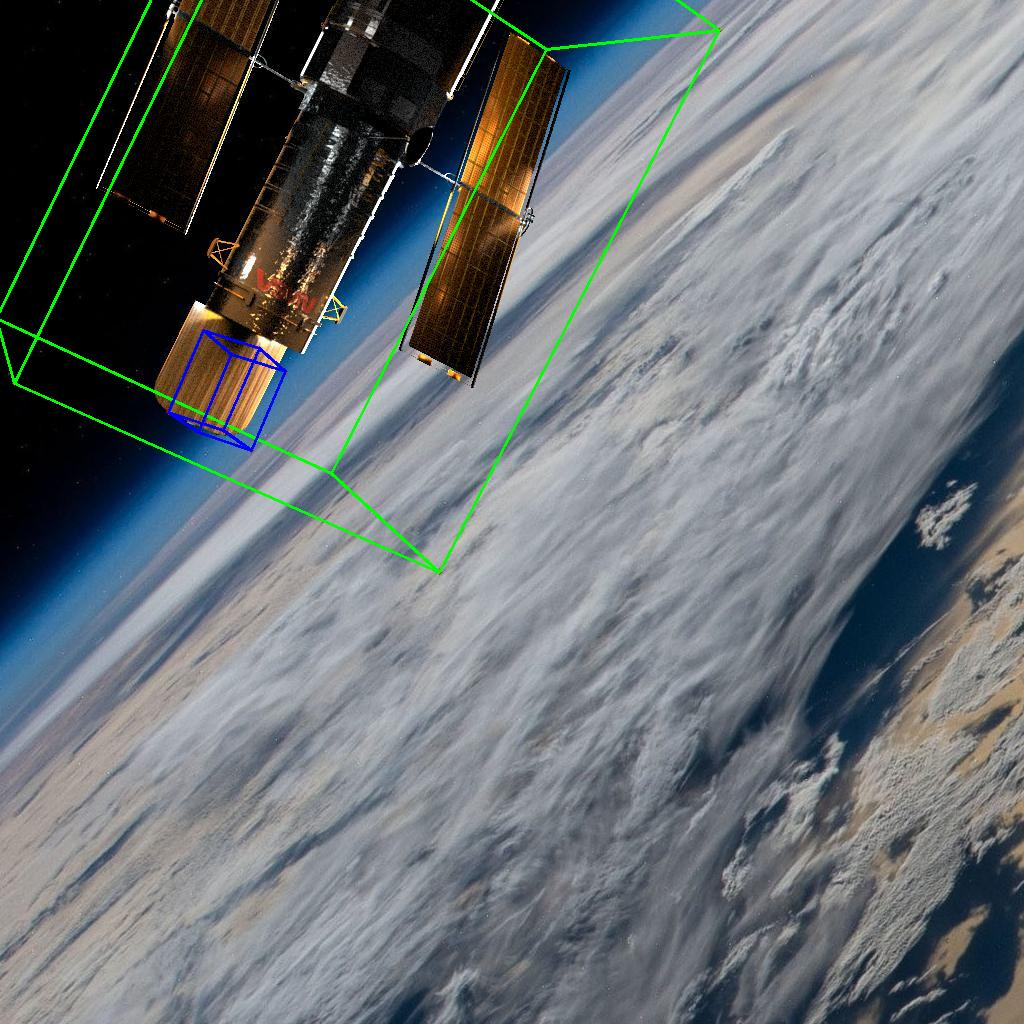
\includegraphics[width=0.70\linewidth]{data/fig1.jpg}
    \caption{Hubble Space Telescope with earth rendered background, 1024x1024 query image number 2, poor pose estimation (blue 3D bounding box) when the object inside the query image is too big.}
    \label{fig:fig1}
\end{figure}
